%%%%%%%%%%%%%%%%%%%%%%%%%%%%%%%%%%%%%%%%%%%%%%%%%%%%%%%%%%%%%%%%%%%%%%%
% Operations Research project report
% Layout follows coa-project-report-ref.tex; subject matter is revised.
%%%%%%%%%%%%%%%%%%%%%%%%%%%%%%%%%%%%%%%%%%%%%%%%%%%%%%%%%%%%%%%%%%%%%%%
\documentclass[12pt,a4paper]{report}

\usepackage[a4paper, margin=1in]{geometry}
\usepackage{graphicx}
\usepackage{fontspec}
\setmainfont{Times New Roman}
\setlength{\emergencystretch}{3em}
\usepackage{amsmath, amssymb}
\usepackage{parskip}
\usepackage[english]{babel}
\usepackage{microtype}
\usepackage{float}
\usepackage{url}
\hyphenation{stand-alone frame-work-less non-func-tion-al high-fi-del-i-ty pre-fetch-ing micro-ar-chi-tec-ture}
\usepackage{hyperref}
\usepackage{tabularx}
\usepackage{booktabs}
\usepackage{fancyhdr}
\usepackage{sectsty}
\usepackage[toc,page]{appendix}
\usepackage{tocbibind}
\usepackage{listings}
\usepackage{xcolor}
\setlength{\headheight}{15pt} % Sized for the Times New Roman header metrics

\definecolor{nordlightbg}{HTML}{ECEFF4}
\definecolor{nordlightfg}{HTML}{2E3440}
\definecolor{nordlightcomment}{HTML}{4C566A}
\definecolor{nordlightkeyword}{HTML}{5E81AC}
\definecolor{nordlightstring}{HTML}{A3BE8C}
\definecolor{nordlightnumber}{HTML}{B48EAD}
\lstdefinestyle{nordlightstyle}{backgroundcolor=\color{nordlightbg},commentstyle=\color{nordlightcomment}\itshape,keywordstyle=\color{nordlightkeyword}\bfseries,numberstyle=\tiny\color{nordlightnumber},stringstyle=\color{nordlightstring},basicstyle=\ttfamily\footnotesize\color{nordlightfg},breakatwhitespace=false,breaklines=true,captionpos=b,keepspaces=true,numbers=left,numbersep=5pt,showspaces=false,showstringspaces=false,showtabs=false,tabsize=2}
\lstset{style=nordlightstyle}

\hypersetup{
    colorlinks=true,
    linkcolor=black,
    citecolor=black,
    urlcolor=black,
    pdftitle={Project Report: Stochastic Traffic Signal Timing Optimization},
    pdfauthor={Dijith Dinesh, Athuljith S, Peter Joe Menachery, Pranav Manoj},
    pdfpagemode=FullScreen,
}
\chapterfont{\centering}
\pagestyle{fancy}
\fancyhf{}
\fancyhead[L]{Stochastic Traffic Signal Timing}
\fancyhead[R]{\nouppercase{\leftmark}}
\fancyfoot[C]{\thepage}
\fancyfoot[L]{Dept. Computer Engineering, MEC 2026}
\renewcommand{\headrulewidth}{0.4pt}
\renewcommand{\footrulewidth}{0.4pt}

\begin{document}
\renewcommand{\bibname}{References}

\begin{titlepage}
\centering
\pagestyle{empty}
\vspace*{0.5cm}
{\Huge\bfseries Stochastic Traffic Signal Timing Optimization\par}
\vspace{0.4cm}
{\large\textbf{PBCBT504: Operations Research Project Report}\par}
\vfill
{\large\itshape Submitted by:\par}
\vspace{0.5cm}
\begin{center}\begin{tabular}{l r}
\bfseries Athuljith S & \bfseries MDL24CSBS021\\
\bfseries Dijith Dinesh & \bfseries MDL24CSBS023\\
\bfseries Peter Joe Menachery & \bfseries MDL24CSBS048\\
\bfseries Pranav Manoj & \bfseries MDL24CSBS049
\end{tabular}\end{center}
\vfill

\includegraphics[width=0.15\textwidth]{college-emblem.png}\par
\vspace{0.5cm}
{\Large\bfseries Department of Computer Engineering\par}
{\large\bfseries Govt. Model Engineering College, Thrikkakara\par}
{\large Ernakulam, Kochi 682021\par}
{\large\href{https://www.mec.ac.in}{https://www.mec.ac.in}\par}
\vspace{1cm}
{\large October 2026\par}
\end{titlepage}

\newpage
\pagestyle{empty}
\begin{center}
{\Large\bfseries Model Engineering College, Thrikkakara\par}
{\large\bfseries Department of Computer Engineering\par}
\vspace{0.4cm}

\includegraphics[width=0.15\textwidth]{college-emblem.png}\par
\vspace{0.4cm}
{\Huge\bfseries CERTIFICATE\par}
\vspace{0.5cm}
\end{center}
\noindent This is to certify that the project report entitled
\large{\bfseries ``Stochastic Traffic Signal Timing Optimization''}
\noindent is a record of the work carried out by
\begin{center}\begin{tabular}{l r}
\bfseries Athuljith S & MDL24CSBS021\\
\bfseries Dijith Dinesh & MDL24CSBS023\\
\bfseries Peter Joe Menachery & MDL24CSBS048\\
\bfseries Pranav Manoj & MDL24CSBS049
\end{tabular}\\
\textbf{Fifth Semester B.Tech Computer Science \& Business Systems}
\end{center}
\noindent students, in partial fulfillment of the requirements for the course \textbf{PBCBT504: Operations Research}.

\noindent The course forms part of the Bachelor of Technology programme of \textbf{APJ Abdul Kalam Technological University}.
\vfill
\begin{tabular}{p{0.45\textwidth}p{0.45\textwidth}}
\hrulefill & \hfill\hrulefill\\
\textbf{Project Guide} & \hfill\textbf{Head of the Department}\\
Signature and name & \hfill Signature and name
\end{tabular}
\vspace{0.5cm}
\begin{center}\hrulefill\\\textbf{Project Coordinator}\\Signature and name\end{center}
\vspace{0.5cm}
\begin{flushleft}Date: \rule{3cm}{0.4pt}\end{flushleft}
\newpage

\chapter*{Acknowledgements}
\thispagestyle{fancy}
We thank the faculty of the Department of Computer Engineering, Government Model Engineering College, for their guidance in framing this as an Operations Research study. The course material on queues, stochastic arrivals, and simulation provided the academic basis for the work. We also thank those who reviewed the problem formulation and helped us distinguish a reproducible simulation result from a field-validated traffic recommendation.

\vspace{0.5cm}
\begin{flushright}{\small\begin{tabular}{l l}
\textbf{Athuljith S} & MDL24CSBS021\\
\textbf{Dijith Dinesh} & MDL24CSBS023\\
\textbf{Peter Joe Menachery} & MDL24CSBS048\\
\textbf{Pranav Manoj} & MDL24CSBS049
\end{tabular}\\[0.2cm]\textbf{Model Engineering College}}\end{flushright}
\newpage

\chapter*{Abstract}
This report studies a finite-horizon traffic signal timing problem using stochastic queuing simulation and constrained enumeration. Four incoming approaches each have dedicated left-turn, through, and right-turn queues. Vehicle arrivals follow independently configured homogeneous Poisson processes; turning movements are sampled at fixed probabilities. A seeded linear congruential generator supplies uniform pseudorandom values, and exponential inverse-transform sampling creates arrival timestamps. A discrete-event engine applies first-come, first-served service with two-second headways during four protected phases and no service during clearance.

The decision is the integer-second green allocation within a fixed 96-second cycle. The objective is expected cumulative waiting, measured as the integrated waiting-queue population across all twelve lanes in a specified operating period. Candidate allocations are evaluated on shared training traffic; the selected allocation and simple baselines are evaluated on separate, matched fresh scenarios. For hypothetical demand of 1,800 vehicles/hour and a ten-minute, empty-start horizon, a four-second-grid search selected 28/16/24/12 seconds for North/East/South/West. Its fresh mean waiting was 10,507.8 vehicle-seconds per run (pointwise 95\% interval 10,430.7--10,584.9). The paired saving against the entered timing was 104.2 vehicle-seconds per run (95\% interval 69.6--138.8). The selected plan equals a demand-proportional baseline on this grid.

A one-second-grid search gives a further but small 0.42\% matched improvement. Heavy demand exceeds the modeled straight-lane capacity under every feasible reallocation, while a 32-minute comparison does not resolve the ten-minute timing advantage. These results are conditional on synthetic rates and simplified geometry; measured traffic data would be needed before a real-world recommendation.
\newpage

\pagenumbering{roman}
\pagestyle{fancy}
\tableofcontents
\newpage
\listoffigures
\newpage
\listoftables
\newpage
\cleardoublepage
\pagenumbering{arabic}

%%%%%%%%%%%%%%%%%%%%%%%%%%%%%%%%%%%%%%%%%%%%%%%%%%%%%%%%%%%%%%%%%%%%%%%
\chapter{Introduction}
%%%%%%%%%%%%%%%%%%%%%%%%%%%%%%%%%%%%%%%%%%%%%%%%%%%%%%%%%%%%%%%%%%%%%%%
\section{Problem Statement}
A fixed-cycle signal shares limited green time among competing approaches, while random arrivals make queues and waiting vary between runs. This study asks which feasible green allocation minimizes expected cumulative waiting over a finite operating period. It models a four-approach junction with dedicated turn lanes, empty initial queues, and a ten-minute primary horizon; it uses synthetic demand and excludes field calibration, pedestrians, and downstream spillback.

\section{Context, Significance, and Objectives}
Signal timing affects waiting, throughput, and queue persistence. Equal green can misallocate capacity when demand differs, while optimization may offer only a small gain over a demand-based rule. Operations Research supplies a disciplined way to compare constrained decisions using queueing and simulation \cite{taha,saaty}. The project formulates this finite-horizon objective, implements a reproducible Rust discrete-event model, exhaustively compares feasible timings on selected grids, evaluates demand and horizon sensitivity, and presents the evidence and limitations in a browser application.

%%%%%%%%%%%%%%%%%%%%%%%%%%%%%%%%%%%%%%%%%%%%%%%%%%%%%%%%%%%%%%%%%%%%%%%
\chapter{System Study}
%%%%%%%%%%%%%%%%%%%%%%%%%%%%%%%%%%%%%%%%%%%%%%%%%%%%%%%%%%%%%%%%%%%%%%%
\section{Physical Scenario and Queue Structure}
Four approaches (N/E/S/W) each have dedicated left, straight, and right FCFS queues. Turns exit onto the next road (from North: left/east, straight/south, right/west; same rotation elsewhere). Three lanes serve during their protected phase; clearance stops service. Capacity follows FHWA's green-share relation \cite{fhwa}.

\section{Queueing Assumptions and Data Source}
M/M/1 assumes exponential service at a continuously available server; our deterministic signal-limited service differs, so its waiting formula does not apply directly \cite{saaty,taha}. Little's formula needs compatible long-run measures \cite{little}; we verify finite-run waiting by queue-area integration. The reference experiments use synthetic inputs and describe no named junction.

\begin{table}[H]\centering\caption{Reference experiment inputs}\label{tab:inputs}
\begin{tabular}{lll}\toprule
Parameter & Value & Interpretation\\\midrule
Approach rates N/E/S/W & 600/350/550/300 veh/h & Total 1,800 veh/h\\
Turn probabilities L/S/R & 20/60/20\% & Independently sampled\\
Cycle, clearance & 96 s, 16 s & 80 s green per cycle\\
Green bounds and grid & 8--44 s, 4 s & 415 feasible plans\\
Service, horizon & 2 s; 600 s & Empty initial queues\\
Entered plan; seed & 24/16/24/16 s; 2026 & Reproducible reference\\\bottomrule
\end{tabular}\end{table}

The application also includes a separate data-based demonstration preset from the City of Toronto's \href{https://open.toronto.ca/dataset/traffic-volumes-at-intersections-for-all-modes/}{Multimodal Intersection Turning Movement Counts}. The City-sourced \href{https://www.toraffic.ca/data/intersection-counts}{intersection count table} lists 3,139 vehicles in the September 16, 2026 AM peak hour at Eglinton Avenue East / Victoria Park Avenue. The summary value is an intersection total, so the preset divides it equally among four approaches (784.75 vehicles/hour each) and retains the application's 20/60/20 turn probabilities. Those disaggregations are assumptions, not measured approach or movement counts. This preset is separate from, and was not used in, the reference results in this report. The source is licensed under the Open Government Licence -- Toronto.


%%%%%%%%%%%%%%%%%%%%%%%%%%%%%%%%%%%%%%%%%%%%%%%%%%%%%%%%%%%%%%%%%%%%%%%
\chapter{Software Requirements Specification (SRS)}
%%%%%%%%%%%%%%%%%%%%%%%%%%%%%%%%%%%%%%%%%%%%%%%%%%%%%%%%%%%%%%%%%%%%%%%
\section{System and Software Requirements}
The system accepts a junction scenario and timing-search request, simulates queues reproducibly, reports uncertainty, and displays interpretable OR results. The Rust core runs natively and as WebAssembly; SolidJS, SVG, and Vite Plus provide the browser interface. Batched runs expose progress, and multiple Web Workers can divide large candidate searches. The interface displays engine outputs without changing the mathematical result.

\section{Functional Requirements}
\begin{itemize}
\item Validate demand, turns, signal bounds, and feasible grids.
\item Generate seeded arrivals and turns; simulate events with conservation and queue-area accounting.
\item Enumerate feasible timings on common training scenarios and choose the lowest estimated waiting.
\item Compare the selected plan with references on matched fresh scenarios and report uncertainty.
\item Display the recommendation, units, queue plots, outcome spread, progress, and replay.
\end{itemize}
Identical requests and seeds reproduce results. Summary memory remains bounded as replications grow; the core is independent of rendering, and saved results retain requests and outputs for audit.

%%%%%%%%%%%%%%%%%%%%%%%%%%%%%%%%%%%%%%%%%%%%%%%%%%%%%%%%%%%%%%%%%%%%%%%
\chapter{System Design and Architecture}
%%%%%%%%%%%%%%%%%%%%%%%%%%%%%%%%%%%%%%%%%%%%%%%%%%%%%%%%%%%%%%%%%%%%%%%
\section{Mathematical Model of Arrivals}
For approach $a$, let $\lambda_a$ be vehicles per second. A homogeneous Poisson process has independent exponential inter-arrival times \cite{taha} and satisfies
\begin{equation}
N_a(t)\sim\operatorname{Poisson}(\lambda_a t),\qquad
\P[N_a(t)=k]=\frac{(\lambda_a t)^k e^{-\lambda_a t}}{k!}.
\end{equation}
Independent exponential gaps construct arrival times event by event. For $U\in(0,1)$,
\begin{equation}\label{eq:gap}
\Delta t=-\frac{\ln(1-U)}{\lambda_a}.
\end{equation}
At 600 vehicles/hour, $\lambda=1/6$ vehicles/second and mean gap is six seconds. For $U=0.20$, Equation~\ref{eq:gap} gives $-6\ln(0.8)=1.34$ seconds. A second uniform draw assigns a turn using the configured cumulative probabilities. Thus a 20/60/20 split is random, not a fixed count of vehicles.

The linear congruential generator uses
\begin{equation}
x_{n+1}=(6364136223846793005x_n+1442695040888963407)\bmod 2^{64}.
\end{equation}
The upper 52 state bits produce a uniform value strictly inside $(0,1)$. A full-period state recurrence does not prove independent random outputs; this is a reproducible simulation source with known limitations.

\section{Discrete-Event State Machine}
For each movement lane, the state stores an FCFS waiting queue, a busy/idle service indicator, arrival and departure counts, maximum waiting population, and the integral of waiting population over time. Events are arrival, green start/end, and service completion. Service starts only if the lane is permitted and its two-second completion fits inside green. A completion at green end is valid. Clearance admits no new service. Equal-time events are ordered completion, green end, green start, arrival, then insertion order.

At each event, the engine first integrates the unchanged queue lengths since the prior event, then applies the state transition. The conservation invariant for each lane $m$ is
\begin{equation}
A_m(t)=D_m(t)+Q_m(t)+S_m(t),\qquad m=1,\ldots,12,
\end{equation}
where $S_m$ is 0 or 1 for in-service population. A scheduled completion beyond the horizon is not counted as a departure by the horizon.

\section{Objective and Complete Formulation}
Let $g=(g_N,g_E,g_S,g_W)$ be integer-second green durations, $C$ the cycle, $L$ total clearance, $T$ observation horizon, and $\omega$ a generated traffic scenario. Waiting population excludes vehicles in service. The single-run objective is
\begin{equation}\label{eq:waiting}
D_T(g,\omega)=\sum_{m=1}^{12}\int_0^T Q_m(t;g,\omega)\,dt
\quad\text{vehicle-seconds}.
\end{equation}
The finite-horizon OR formulation is
\begin{align}
\min_{g\in\Omega}\quad &\mathbb{E}_{\omega}[D_T(g,\omega)]\\
\Omega=\{g\in\mathbb{Z}^4:\quad
&\sum_i g_i=C-L,\quad g_{\min}\le g_i\le g_{\max},\\
&g_i=g_{\min}+k_i\Delta,\quad k_i\in\mathbb{Z}_{\ge0}\}.
\end{align}
The entered plan need not lie on the search lattice, although it must satisfy base timing constraints. In the reference case $C-L=80$ seconds, $g_{\min}=8$ seconds, and $g_{\max}=44$ seconds. The four-second request has 415 feasible timings. A one-second request has 19,369.

\section{Performance Measures}
Between events, queue area increases by $Q_m(t_{old})(t_{new}-t_{old})$. Mean queue is area/$T$; throughput counts completed departures, and backlog counts vehicles still waiting at $T$. Mean waiting per arrival averages $D_T/A$ across runs, including partial waits at $T$ rather than completed-trip travel time.

%%%%%%%%%%%%%%%%%%%%%%%%%%%%%%%%%%%%%%%%%%%%%%%%%%%%%%%%%%%%%%%%%%%%%%%
\chapter{Implementation}
%%%%%%%%%%%%%%%%%%%%%%%%%%%%%%%%%%%%%%%%%%%%%%%%%%%%%%%%%%%%%%%%%%%%%%%
\section{Rust/WASM Engine and Experiment Pipeline}
The Rust core separates deterministic queue transitions, scenario generation, and experiment orchestration. It generates seeded Poisson scenarios, enumerates feasible timings against common training arrivals, then evaluates the selected and reference plans on matched fresh arrivals.

The Rust engine has four crates: replaceable random generation, queue simulation, experiment orchestration, and a WebAssembly adapter. Each event applies $S_{n+1}=F(S_n,e_n,c)$ to explicit state and configuration, returning the next state without external I/O. The experiment session is a state machine that advances through training, fresh evaluation, optional sensitivity analysis, and completion.

The request fixes the 64-bit linear congruential generator seed. The same request and engine build reproduce the scenarios, and candidate plans replay the same arrivals for fair comparison. Batch size does not change the result. This supports audit and replay, but does not establish statistical independence or validate assumed traffic rates.

The Rust model compiles to the browser's \path{wasm32-unknown-unknown} target through \path{wasm-bindgen} \cite{rust-wasm,wasm-bindgen}. A worker advances bounded batches and reports progress to SolidJS. Large searches (at least 20,000 candidate--scenario evaluations) can split candidate ranges across up to 16 dedicated Web Workers, each running its own WASM instance; the coordinator merges statistics and one worker performs fresh evaluation. This is worker-level parallelism, not shared-memory WASM threading \cite{html-workers}. Graphs and animation display engine outputs and do not define the objective.

Batching exposes live progress. Queue profiles, moments, and density grids are accumulated without retaining every vehicle trace; selected traces can be regenerated for playback.

\section{Optimization and Application}
After validating the request, the engine enumerates feasible $g$, scores each plan on common training scenarios, selects the lowest sample mean $D_T$, then compares the selected and reference plans on matched fresh scenarios. It reports timing, total and per-arrival waiting, queue profiles, residual backlog, and uncertainty. SolidJS renders SVG graphs and lane-correct replay from WASM results; the animation does not alter the objective. The public application is \url{https://traffic-signal-analysis.pages.dev/} \cite{web}.

For paired comparison, a replication's saving is
\begin{equation}
d_r=D_T(g_{\mathrm{reference}},\omega_r)-D_T(g_{\mathrm{selected}},\omega_r).
\end{equation}
Positive $d_r$ favors the selected plan. Welford's updates accumulate means and sample variances. A pointwise approximate 95\% interval is
\begin{equation}
\bar d\pm t_{0.975,R-1}\frac{s_d}{\sqrt R}.
\end{equation}
The paired-mean interval follows the usual Student-$t$ form \cite{taha}. These intervals describe sampling variation conditional on the model. They do not measure uncertainty about field conditions or give a simultaneous guarantee over all searched timings.

\begin{figure}[H]\centering
\begin{minipage}{0.48\textwidth}\centering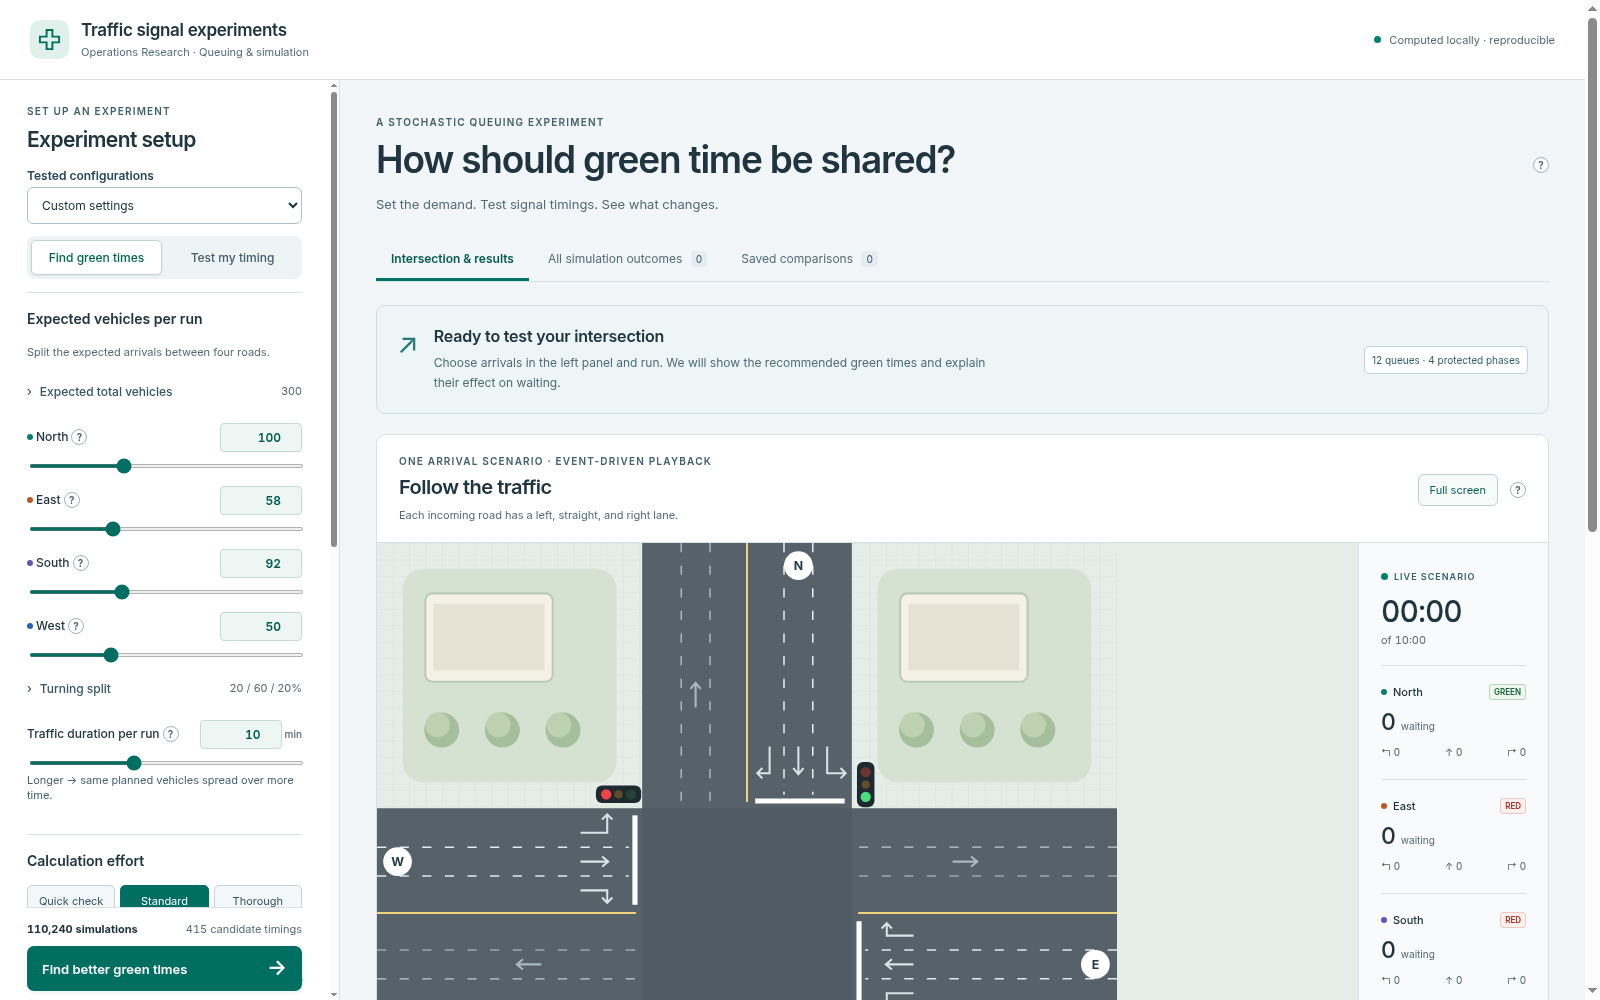
\includegraphics[width=\textwidth]{assets/ui-setup.png}\end{minipage}\hfill
\begin{minipage}{0.48\textwidth}\centering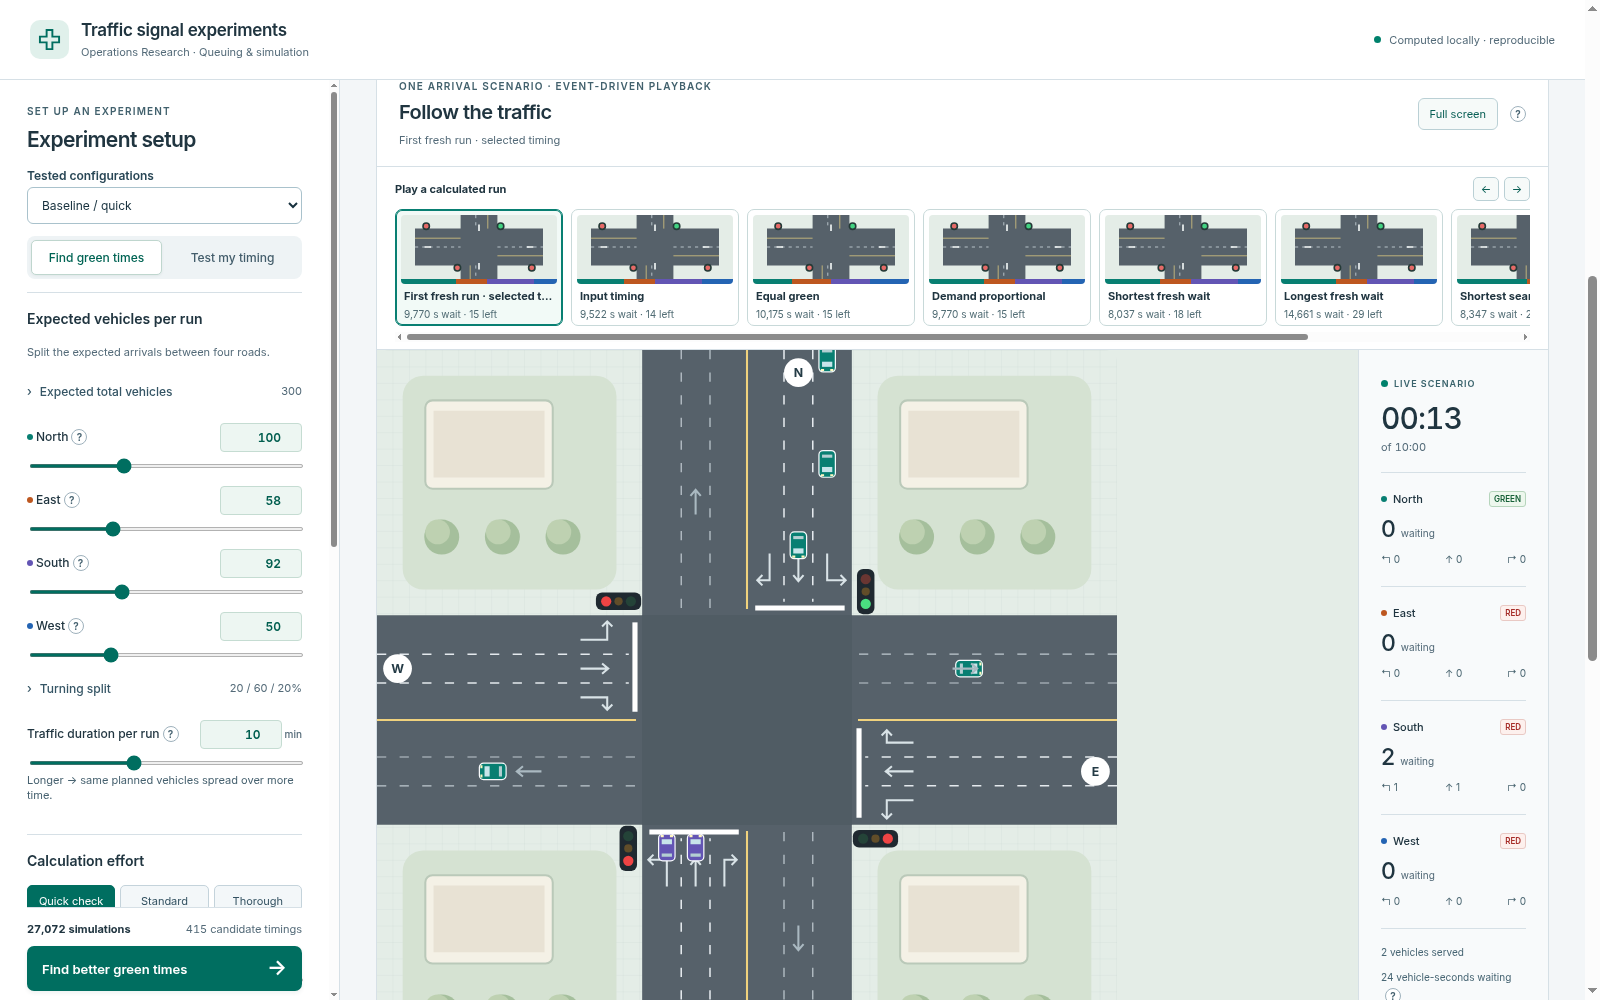
\includegraphics[width=\textwidth]{assets/ui-simulation.png}\end{minipage}
\caption{Browser application: scenario controls (left) and signal/vehicle replay (right)}\label{fig:ui}
\end{figure}

%%%%%%%%%%%%%%%%%%%%%%%%%%%%%%%%%%%%%%%%%%%%%%%%%%%%%%%%%%%%%%%%%%%%%%%
\chapter{Testing}
%%%%%%%%%%%%%%%%%%%%%%%%%%%%%%%%%%%%%%%%%%%%%%%%%%%%%%%%%%%%%%%%%%%%%%%
\section{Verification and Monte Carlo Convergence}
Tests cover inverse sampling, hand-checked event traces, phase boundaries, lane permissions, vehicle conservation, queue-area integration, grid enumeration, paired statistics, batch invariance, progress, and bounded summaries. An audit checked 23 saved outputs for request/replication consistency and agreement between queue profiles and cumulative waiting.

These checks establish consistency with the model, not field validity. No observed traffic was used to calibrate the assumed Poisson arrivals, turn probabilities, two-second headway, or protected phases. With repeated scenarios, the sample mean approaches the model expectation; individual run delays need not be Gaussian. More runs reduce sampling error but cannot fix incorrect assumptions. Figure~\ref{fig:convergence} shows the running mean for 1,000 fresh runs.

\begin{figure}[H]\centering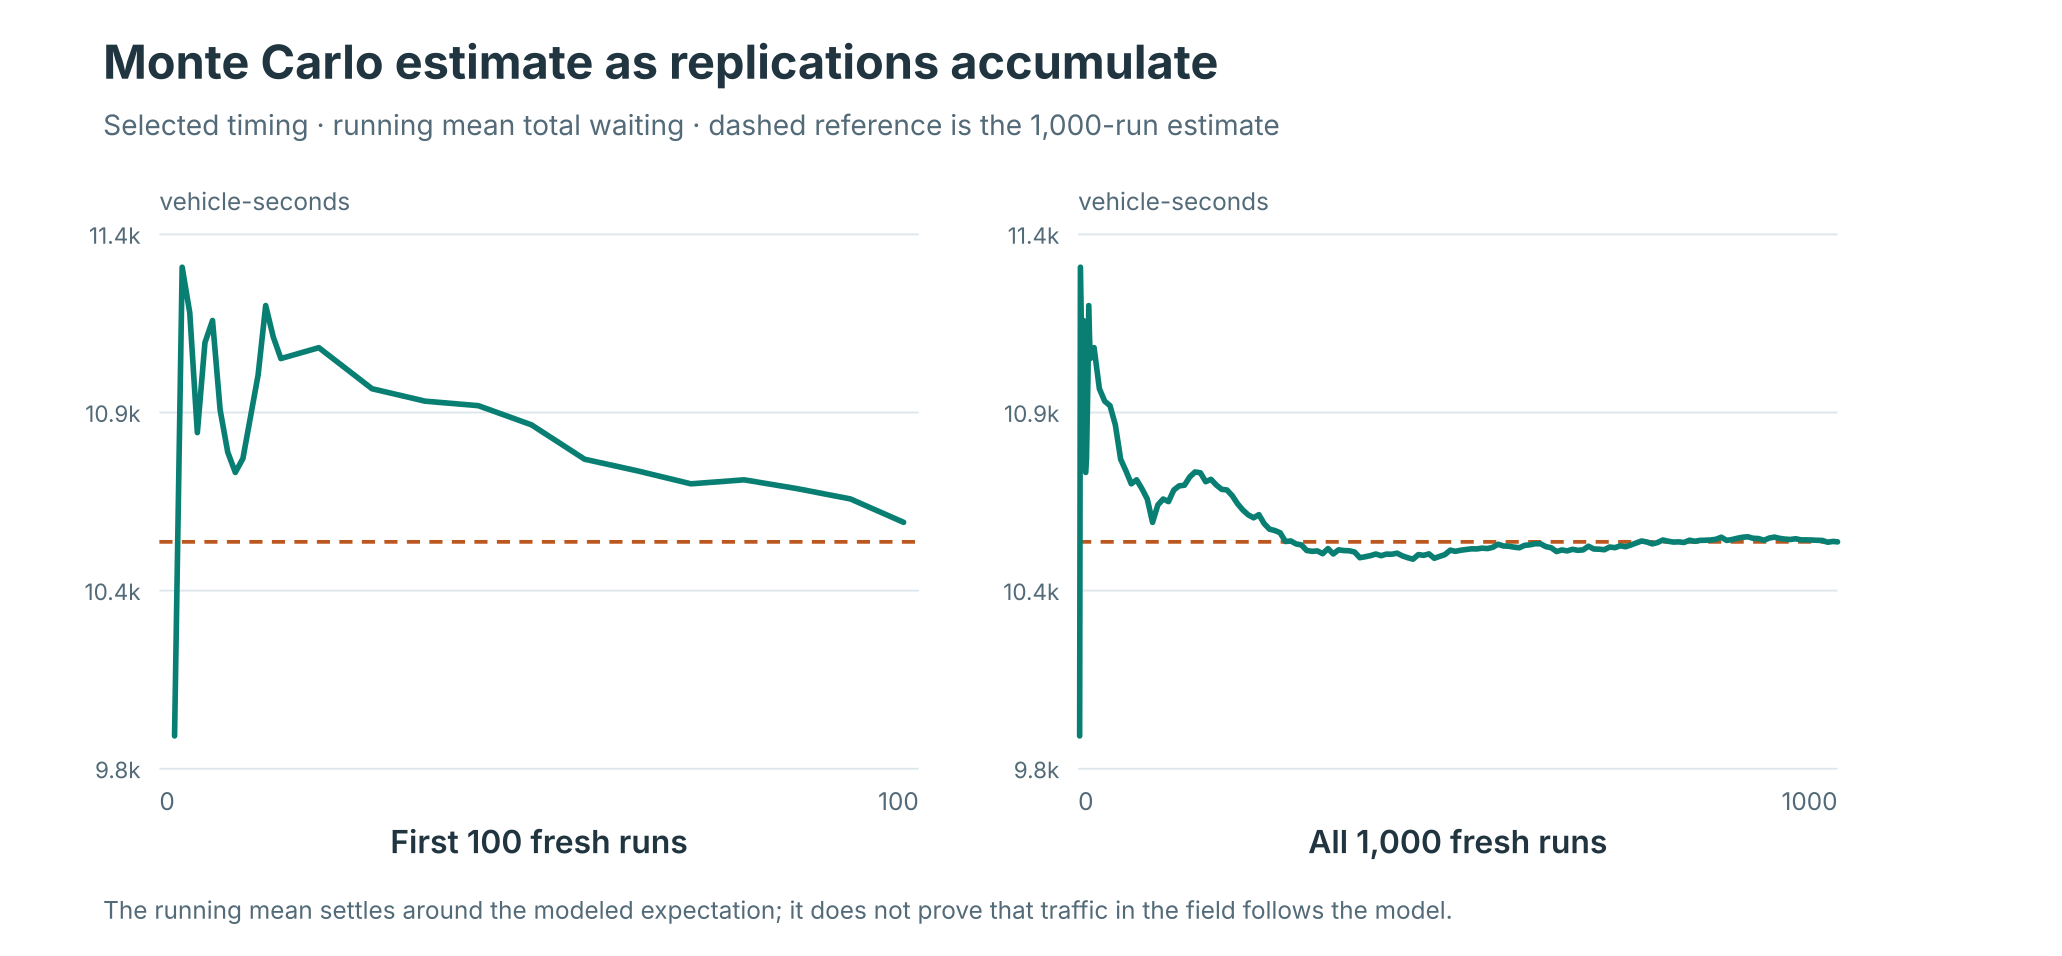
\includegraphics[width=0.75\textwidth]{assets/fig-convergence.png}
\caption{Running mean cumulative waiting over 1,000 fresh reference runs}\label{fig:convergence}\end{figure}

%%%%%%%%%%%%%%%%%%%%%%%%%%%%%%%%%%%%%%%%%%%%%%%%%%%%%%%%%%%%%%%%%%%%%%%
\chapter{Results and Discussion}
%%%%%%%%%%%%%%%%%%%%%%%%%%%%%%%%%%%%%%%%%%%%%%%%%%%%%%%%%%%%%%%%%%%%%%%
\section{Reference Ten-Minute Result}
At the baseline synthetic rates, the four-second grid contains 415 feasible timings. Each was scored on 256 shared training scenarios. The selected 28/16/24/12-second split was evaluated with 1,000 fresh scenarios, together with three reference plans. Table~\ref{tab:mainresults} gives the principal result.

\begin{table}[H]\centering\caption{Principal fresh-evaluation result, ten-minute reference case}\label{tab:mainresults}
\begin{tabular}{ll}\toprule
Measure & Value\\\midrule
Selected green N/E/S/W & 28/16/24/12 s\\
Mean total waiting & 10,507.8 vehicle-s/run\\
Pointwise 95\% interval & 10,430.7--10,584.9 vehicle-s/run\\
Mean observed waiting per arrival & 35.08 s\\
Mean end waiting population & 18.77 vehicles\\
Input minus selected paired saving & 104.2 vehicle-s/run\\
Paired 95\% interval & 69.6--138.8 vehicle-s/run\\\bottomrule
\end{tabular}\end{table}

The selected allocation equals the grid-projected demand-proportional baseline. Its gain over the entered timing is statistically resolved within this model but modest: about 0.35 seconds per expected arrival. The objective value is cumulative vehicle-seconds, not vehicles per second and not average seconds per completed trip.

\begin{figure}[H]\centering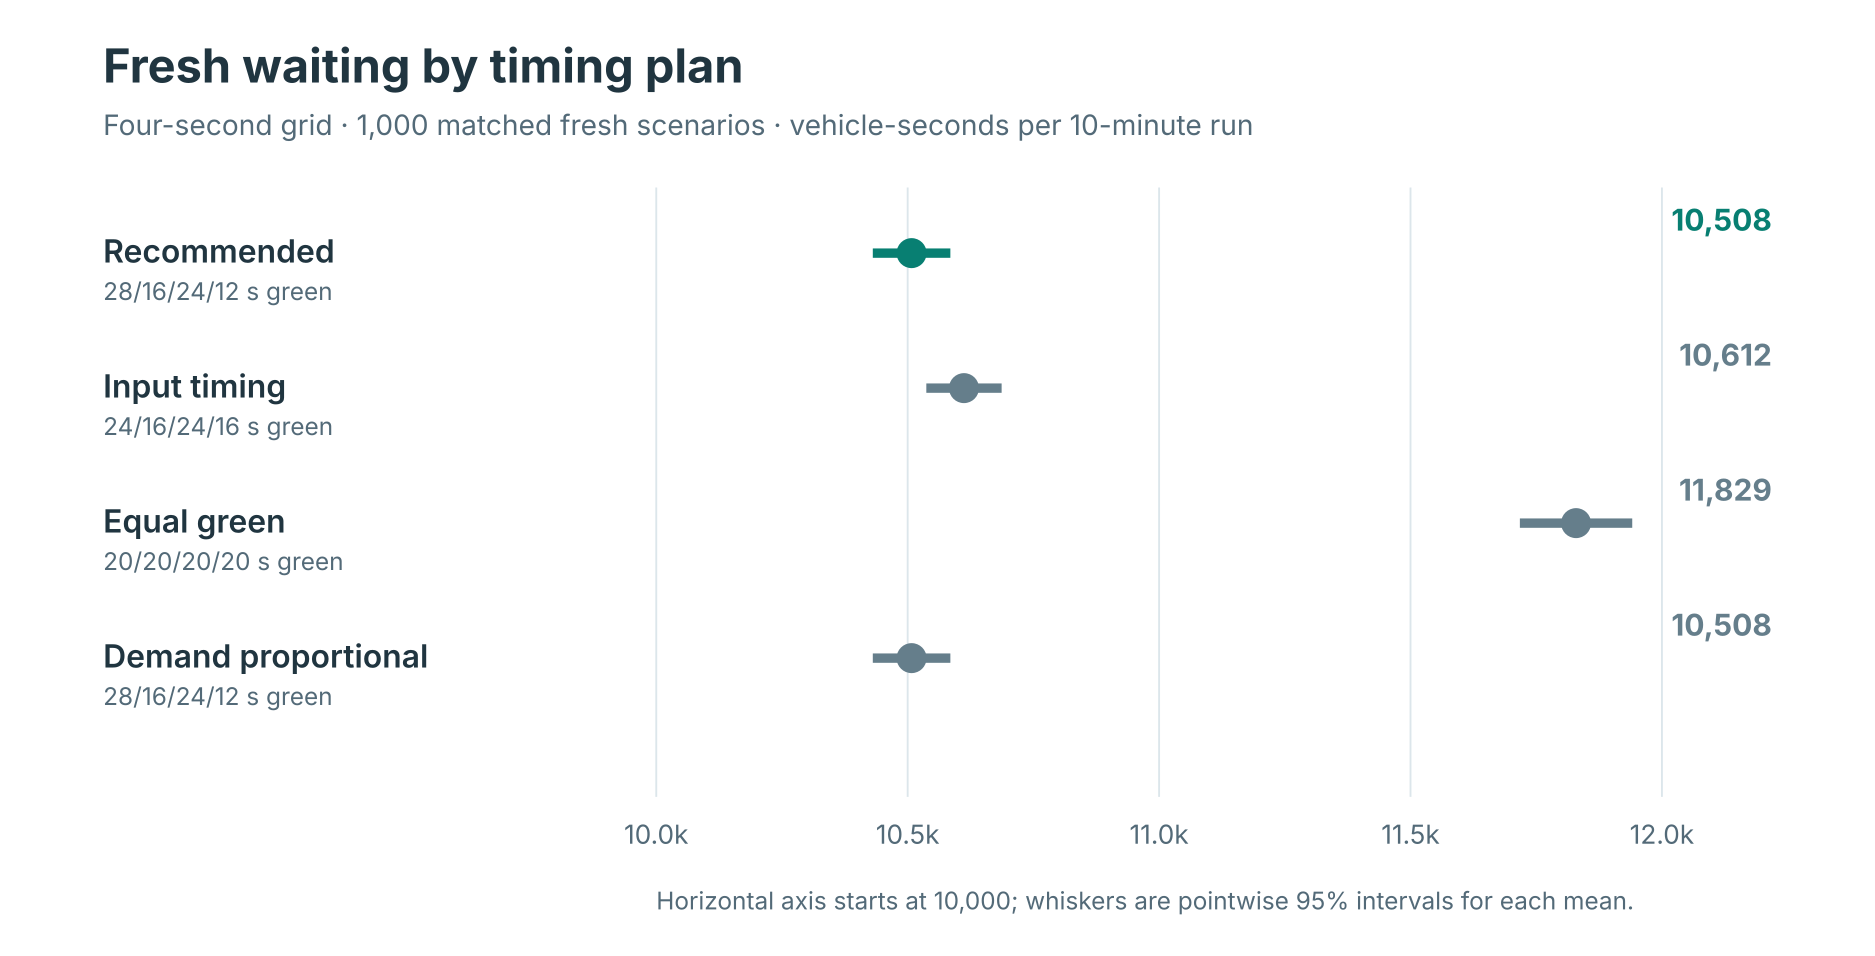
\includegraphics[width=0.75\textwidth]{assets/fig-timing.png}
\caption{Fresh mean waiting for selected and reference timings; lower is better}\label{fig:timing}\end{figure}

\section{Mean Queue Behavior}
Figure~\ref{fig:queues} displays the mean waiting population by incoming approach over 1,000 fresh runs at the selected timing. Each point represents a short interval average, not one arbitrary example run. The combined area of the four curves equals the fresh mean total waiting within numerical precision. Vehicles still waiting at 600 seconds have contributed partial waiting.

\begin{figure}[H]\centering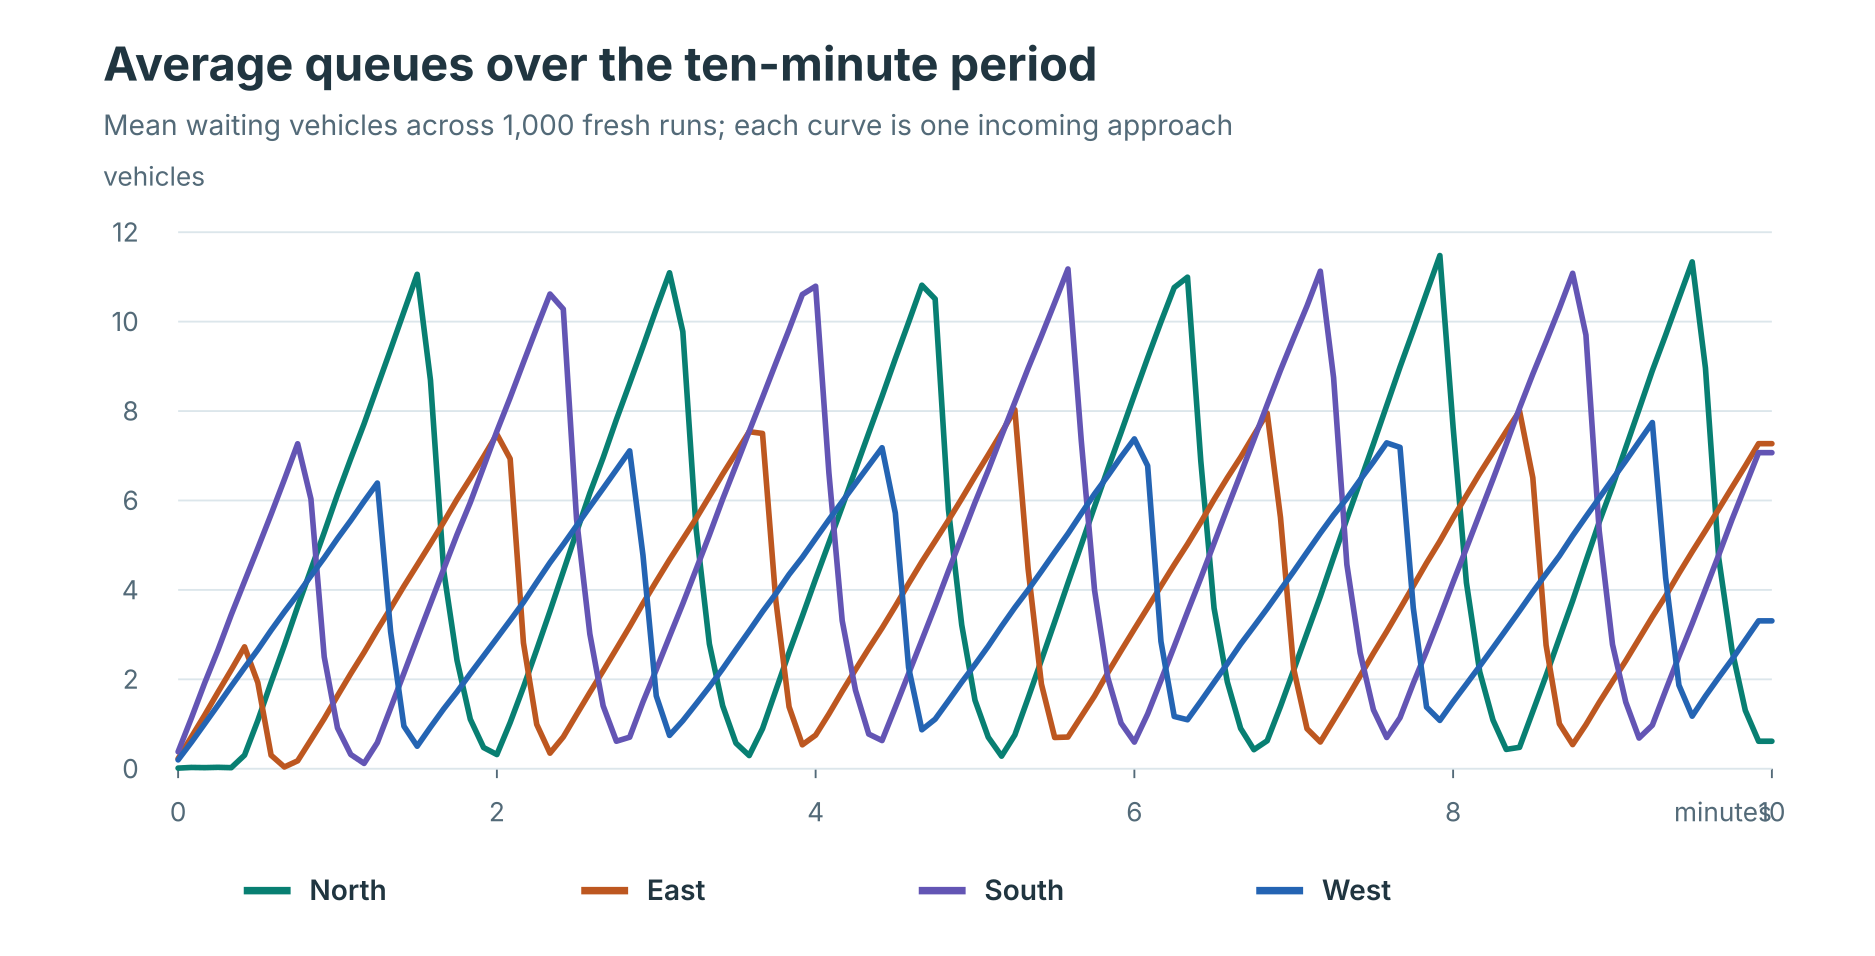
\includegraphics[width=0.75\textwidth]{assets/fig-queues.png}
\caption{Average waiting queues by approach over the ten-minute period}\label{fig:queues}\end{figure}

\section{Fine-Grid Search and Runtime}
The one-second grid contains 19,369 feasible allocations. The original native study search used 128 training runs per candidate and finished in 209.02 seconds. The optimized Rust engine reran the same request in 6.86 seconds (30.5 times faster) and selected the same timing, 26/16/24/14 seconds. A separate 5,000-run evaluation gave 10,495.0 vehicle-seconds/run, with a pointwise 95\% interval of 10,462.8--10,527.2. On the same 5,000 fresh scenarios, it saved 44.8 vehicle-seconds/run over the four-second-grid selection (paired 95\% interval 34.8--54.8), or 0.42\% of the coarse plan's mean. The speedup comes from reusing independent approach/phase simulations; it does not change the modeled objective.

Three additional matched seed checks each used 5,000 scenarios and favored the finer fixed plan, with savings of 46.4, 46.8, and 56.0 vehicle-seconds/run. The searches had different training counts; the result supports a small advantage of these two fixed plans for this ten-minute model, not proof of a global expected-value optimum.

Table~\ref{tab:runtime} preserves the original-study wall-clock times for each complete main-study request when executed by the native release-mode Rust study program on the study machine. A request includes its timing search, fresh evaluation, and configured sensitivity work; the figures are not per-simulation costs. The optimized backend timings above are a separate post-study comparison. Neither set benchmarks the browser's WebAssembly workers or should be extrapolated to other hardware or to a million-replication run.

\begin{table}[H]\centering\caption{Original-study native runtime for each principal study request}\label{tab:runtime}
\begin{tabular}{lrrr}\toprule
Study case & Grid & Search/fresh runs & Runtime (s)\\\midrule
Baseline quick & 4 s & 64/128 & 2.45\\
Baseline reference & 4 s & 256/1,000 & 10.27\\
Baseline precise & 4 s & 256/5,000 & 11.39\\
Quiet reference & 4 s & 256/1,000 & 4.92\\
Heavy reference & 4 s & 256/1,000 & 14.67\\
South-heavy reference & 4 s & 256/1,000 & 9.54\\
Fine-grid verification & 1 s & 128/5,000 & 209.02\\\bottomrule
\end{tabular}\end{table}

The separate matched comparison of the coarse and fine selected plans took 1.25 seconds natively. The additional seed and horizon audit checks were not individually timed in the retained records, so no runtimes are claimed for them. These times are computational costs, not optimization objective values; waiting results remain the basis for the OR decision.

\section{Demand, Capacity, and Horizon Sensitivity}
Table~\ref{tab:demand} reports separately re-optimized synthetic scenarios. South-heavy demand keeps the total rate unchanged but shifts allocation toward South. Direct cumulative-waiting comparisons across 150, 300, and 450 expected arrivals also change workload, so they are not pure timing benefits.

\begin{table}[H]\centering\caption{Re-optimized four-second-grid demand scenarios}\label{tab:demand}
\begin{tabular}{lrrrr}\toprule
Scenario & Exp. arrivals & Green N/E/S/W & Waiting (veh-s) & End backlog\\\midrule
Quiet & 150 & 36/12/20/12 & 4,580.6 & 8.27\\
Reference & 300 & 28/16/24/12 & 10,507.8 & 18.77\\
Heavy & 450 & 28/16/24/12 & 23,431.5 & 54.40\\
South-heavy & 300 & 16/16/36/12 & 10,077.9 & 18.50\\\bottomrule
\end{tabular}\end{table}

At the selected reference split, heavy straight demand is 540, 315, 495, and 270 vehicles/hour for North, East, South, and West. Ideal per-lane capacities are 525, 300, 450, and 225 vehicles/hour, respectively.

Even without integer rounding, those four straight streams require 86.4 green seconds per cycle, more than the available 80. No feasible reallocation can serve all heavy straight demand under this model. Mean end backlog grows from 54.4 vehicles at ten minutes to 110.1 at 32 minutes. This is a structural capacity limit, not a failure of timing search.

The principal 600-second horizon ends after 6.25 signal cycles. Its endpoint and empty initial queues are part of the objective. Re-optimization selected 28/16/24/12 seconds at 576, 600, 624, 672, and 960 seconds, but 24/16/24/16 seconds at 1,920 seconds. To isolate the timing effect, 5,000 fresh matched scenarios per horizon compared the two fixed plans (seed 2027).

\begin{table}[H]\centering\caption{Paired saving of 28/16/24/12 s against 24/16/24/16 s}\label{tab:horizon}
\begin{tabular}{rrr}\toprule
Horizon & Mean saving (vehicle-s/run) & Paired 95\% interval\\\midrule
600 s & 105.5 & 88.5--122.5\\
960 s & 64.0 & 35.8--92.2\\
1,920 s & 15.0 & $-40.3$--70.2\\\bottomrule
\end{tabular}\end{table}

The 32-minute interval includes both signs; there is no resolved advantage at that horizon. The recommendation must therefore remain specific to the ten-minute experiment. Total vehicle-seconds from unequal horizons cannot be compared directly as if the exposure were identical.

%%%%%%%%%%%%%%%%%%%%%%%%%%%%%%%%%%%%%%%%%%%%%%%%%%%%%%%%%%%%%%%%%%%%%%%
\chapter{Conclusion and Future Scope}
%%%%%%%%%%%%%%%%%%%%%%%%%%%%%%%%%%%%%%%%%%%%%%%%%%%%%%%%%%%%%%%%%%%%%%%
\section{Conclusion}
In the ten-minute synthetic case, the four-second search selected 28/16/24/12 seconds; mean waiting was 10,507.8 vehicle-seconds per run. It tied the demand-based plan and modestly improved on the entered timing. The finer grid improved mean waiting by 0.42\%. Under heavy demand, modeled capacity was exceeded; at 32 minutes, the timing advantage was unresolved.

\section{Limitations}
Results depend on synthetic Poisson rates, fixed turns, dedicated lanes, deterministic service, protected phases, empty initial queues, and the chosen horizon. No field calibration was performed; intervals quantify simulation variation conditional on these assumptions and do not prove real-world optimality.

\section{Future Scope}
\begin{enumerate}
\item Collect approach counts, turn proportions, headways, and observed queues, then calibrate against held-out periods.
\item Extend the model to platoons, pedestrians, shared lanes, downstream storage, and alternative phase structures.
\item Validate predicted queues and waiting against field observations before making operational recommendations.
\end{enumerate}

\begin{thebibliography}{10}
\bibitem{taha} H. A. Taha, \emph{Operations Research: An Introduction}, 10th ed. Pearson, 2017. \href{https://www.pearson.com/en-gb/subject-catalog/p/Taha-Operations-Research-An-Introduction-Global-Edition-10th-Edition/P200000005533}{Online}.
\bibitem{saaty} T. L. Saaty, \emph{Elements of Queuing Theory, with Applications}. New York: McGraw--Hill, 1961. \href{https://books.google.com/books?id=NdI-AAAAIAAJ}{Online}.
\bibitem{little} J. D. C. Little, ``A Proof for the Queuing Formula: $L=\lambda W$,'' \emph{Operations Research}, vol. 9, no. 3, pp. 383--387, 1961. \href{https://doi.org/10.1287/opre.9.3.383}{Online}.
\bibitem{fhwa} Federal Highway Administration, \emph{Traffic Signal Timing Manual}, Chapter 3, FHWA-HOP-08-024. \href{https://ops.fhwa.dot.gov/publications/fhwahop08024/chapter3.htm}{Online}.
\bibitem{rust-wasm} Rust Project, \emph{The rustc book: wasm32-unknown-unknown Target}. \href{https://doc.rust-lang.org/rustc/platform-support/wasm32-unknown-unknown.html}{Online}.
\bibitem{wasm-bindgen} Rust WebAssembly Working Group, \emph{The wasm-bindgen Guide}. \href{https://wasm-bindgen.github.io/wasm-bindgen/}{Online}.
\bibitem{html-workers} WHATWG, \emph{HTML Living Standard: Web Workers}. \href{https://html.spec.whatwg.org/multipage/workers.html}{Online}.
\bibitem{web} Project team, \emph{Traffic Signal Analysis: Interactive Simulation Application}, 2026. \href{https://traffic-signal-analysis.pages.dev/}{Online}.
\end{thebibliography}

\end{document}
